% !TeX root=../main.tex

\chapter{مقدمه}
% دستور زیر باعث عدم‌نمایش شماره صفحه در اولین صفحهٔ این فصل می‌شود.
\thispagestyle{empty}
\section{پیشگفتار}
یک سیستمِ احراز هویت به‌وسیله چهره را در نظر بگیرید که کاربر در مقابل دوربین قرار گرفته و سیستم از طریق تایید مشخصات چهره، به او اجازه دسترسی می‌دهد. حال فرض کنید کاربر غیر مجاز تصویر کاربرِ قبلاً تایید شده در سیستم را روی کاغذ چاپ کند و کاغذ را در مقابلِ دوربینِ سیستم قرار دهد. در این صورت کاربر غیر مجاز می‌تواند خود را به‌جای کاربر مجاز به سیستم بشناساند و به اطلاعات محرمانه فرد دیگری، به کمک تنها یک تصویر چاپ شده، دسترسی پیدا کند. این یک مثال ساده برای تداعی مشکل امنیتی سیستم‌های احراز اصالت با چهره است.

هر چه محرمانگی و اهمیت اطلاعات ذخیره شده درون سیستم بیشتر باشد، مشکل امنیتی ذکر شده توجه بیشتری می‌طلبد. برای مثال فرض کنید سیستم مذبور با اطلاعات حساب بانکی یا اوراق بهادار یا داده‌های محرمانه یک شرکت تجاری مرتبط باشد؛ در این صورت تمامی این اطلاعات حیاتی در معرض خطر آسیب پذیری فرآیند تشخیص و تایید چهره خواهد بود.

این چالش در ادبیات موضوع «جلوگیری از تقلب برای احراز هویت مبتنی بر تشخیص چهره
\LTRfootnote{Anti-spoofing for authentication based on face recognition}
» نام دارد. در این عنوان، قسمت احراز هویت مبتنی بر تشخیص چهره در واقع شاخه از بایومتریک
%\href{Biometric}{}
\LTRfootnote{Biometric}
   است و قسمت جلوگیری از تقلب، به مسائل امنیتی کار می‌پردازد.
هدف از بایومتریک، تشخیص خودکارِ افراد بر اساس ویژگی‌های زیست‌شناختی و یا رفتار اشخاص است. برای مثال چهره، عنبیه، اثر انگشت، صدا و طرز راه رفتن نمونه از ویژگی‌هایی است که هر فرد را به‌صورت منحصراً از فرد دیگر تمیز می‌دهد.  تأکید بایومتریک بر «خودکار بودن» فرآیند تشخیص فرد است؛ به همین دلیل لازم است که دخالت انسان در این فرآیند حداقل شود و سیستم به‌صورت غیر نظارتی
\LTRfootnote{Unsupervised}
 فرد را تشخیص دهد.
در میان شاخصه‌های ذکر شده برای کاربرد بایومتریک، استفاده از چهره اهمیت خاصی دارد. روش‌های بینایی ماشین برای تشخیص چهره سابقه طولانی دارند و به‌تازگی راه حل‌های استفاده از هوش مصنوعی، تشخیص چهره را دقیق‌تر و متداول‌تر کرده است. از طرفی چهره در مقایسه با اثر انگشت یا صدا و... نمایان‌گر آشناتر برای شناسایی یک فرد است. این ویژگی‌های چهره چه در ابزار شناسایی چه در قرابت استفاده، موجب شده است تشخیص چهره، کاربردهای دیگری نظیر پزشکی قانونی، دوربین‌های مدار بسته، اجازه کنترل و دسترسی به سیستم، و دولت و تجارت الکترونیک داشته باشد.


این کاربرد گسترده و رشد استفاده از چهره در سیستم‌ها، مسائل امنیتی را نیز به همراه دارد. مهاجم براحتی و با هزینه‌ی کمی می‌تواند تصویر فرد مورد نظر خود را از طریق شبکه‌های اجتماعی یا تصویر برداری از فاصله دور به‌دست آورد و اقدامات لازم برای حمله را به عمل آورد.
این نوع حمله با ابزارهای مختلفی می‌تواند صورت بگیرد. برای مثال مهاجم می‌تواند تصویر فرد هدف را روی کاغذ چاپ کند، یا از یک فیلم یا تصویر ذخیره شده در نمایشگر دیجیتال استفاده کند. همچنین با استفاده از گریم یا ماسک می‌تواند چهره خود را شبیه به چهره فرد هدف کند. در میان انواع حمله ذکر شده استفاده از چاپ تصویر و استفاده از نمایشگر دیجیتال متداول‌تر است. استفاده از ماسک به‌دلیل هزینه بالا و سختی اجرا، چندان متداول نیست. با توجه به اهمیت موضوع و نگرانی در مورد امنیت سیستم‌های احراز هویت مبتنی بر تشخیص چهره، تحقیقات فراوانی در دانشگاه برای فائق آمدن بر این چالش انجام شده است. که دامنه وسیعی از روش‌های مبتنی بر بینایی ماشین کلاسیک و روش‌های جدیدتر مبتنی بر هوش مصنوعی و یادگیری عمیق را شامل می‌شود.


این مسئله می‌تواند از دید یک مسئله‌ی بینایی ماشین تعریف شود به‌گونه‌ای که ورودی مسئله تصویر از چهره یک فرد است و خروجی سیستم یک برچسب چهره واقعی یا تقلبی است. دقت الگوریتم برای اعلام این برچسب‌گذاری، سهم مهمی در امینت کلی سیستم خواهد داشت. در برخی از روش‌ها از اطلاعات بیشتری نظیر سنسور حرارتی و یا مادون قرمز در کنار تصویر استفاده می‌شود اما این امر موجب افزایش هزینه خواهد شد. همچنین الگوریتم‌ها بر اساس استفاده از تنها یک تصویر یا یک دنباله ویدیویی نیز قابل تقسیم هستند.


با وجود تلاش‌های تحقیقاتی در این زمینه که بیش از یک دهه قدمت دارد همچنان مسئله کشف تقلب در تشخیص چهره یک مسئله چالشی می‌باشد. یکی از دلایل چالشی بودن آن، خلاقیت فرد مهاجم برای اعمال حمله جدید است به‌گونه‌ای که این نوع حمله قبلاً در داده‌های آموزشی شبکه وجود نداشته است. یک چالش دیگر تفاوت کیفیت و رزولوشن ابزارهای حمله، نظیر صفحه نمایش و کاغذ چاپ است. این مسئله زمانی بغرنج‌تر می‌شود که حتی برای کاربر انسانی نیز تمیز چهره واقعی و تقلبی دشوار خواهد شد. برای مثال در شکل 
\ref{fig:realandfake}
یکی از تصاویر تقلبی و دیگری واقعی است. همانطور که مشاهده می‌شود تشخیص چهره واقعی از تقلبی به آسانی میسر نیست.


\begin{figure}[ht]
	\centerline{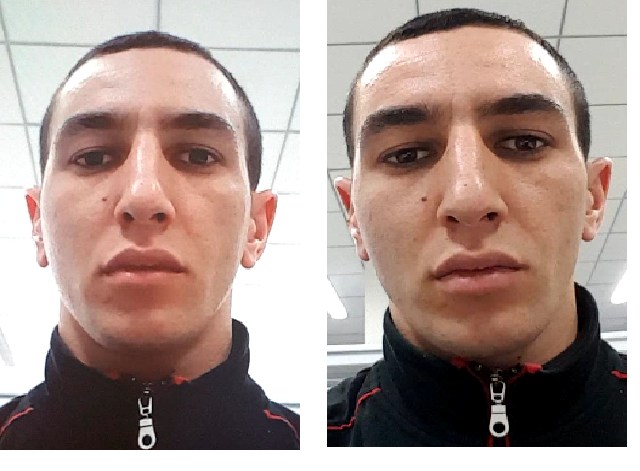
\includegraphics[width=\linewidth]{realAndFakeEx}}
	\caption{نمونه‌ای از تصاویر واقعی و تقلبی در حوزه چهره \cite{boulkenafet2017oulu}}
	\label{fig:realandfake}
\end{figure}

\section{اهداف}
در این پایان‌نامه برای کشف تقلب در تصویر چهره، تمرکز بر روش‌هایی است که تنها از تصویر رنگی به‌عنوان ورودی استفاده می‌شود. این رویکرد موجب کاهش هزینه سیستم و قابل استفاده بودن بیشتر خواهد شد. همچنین از انواع حمله‌های مختلف موجود، تنها موارد چاپ روی کاغذ و بازپخش ویدیو بررسی می‌گردد. با آن‌که حمله‌های دیگری نظیر استفاده از ماسک سه بعدی نیز وجود دارد اما اعمال چنین حمله‌هایی هزینه‌بر و دشوارتر از نظر اجرا است. بنابرین توجه پایان‌نامه روی حملاتی است که متداول‌تر و بیشتر قابل اجرا است. در این پایان‌نامه با ترکیب روش کلاسیک بینایی ماشین و روش‌های جدید یادگیری عمیق ساختاری برای طبقه‌بندی دقیق‌تر ارائه شده است. این ساختار شامل یک عملگر جدید است که از عملگر LBP کلاسیک الهام گرفته شده است، با این تفاوت که این عملگر همانند عملگر کانولوشن در شبکه‌های عمیق دارای پارامتر برای یادگیری عملگر بهینه با توجه به داده‌های ورودی است. همچنین دو تابع هزینه جدیدی ارائه شده است که هدف آن افزایش دقت و تعمیم‌پذیری شبکه روی داده‌های آزمون دیده نشده است.
\section{دستاورد‌های پژوهش}
در این پایان‌نامه نشان داده می‌شود روش ارائه شده شامل عملگر تحلیل ریزبافت و تابع هزینه جدید موجب افزایش دقت طبقه‌بندی و تعمیم پذیری آن می‌شود. همچنین برای پیاده‌سازی، برنامه‌نویسی به زبان پایتون انجام شده است و ملاحظات پیاده‌سازی و چالش‌های مربوط به آن، توضیح و تفسیر شده است. علاوه بر این، برای کار کردن با داده‌های ویدیویی و استفاده از آن، الگوریتمی ارائه شده است که روند آموزش شبکه را تسریع ببخشد. کدهای مرتبط با برنامه در یک مخزن گیت‌هاب
\LTRfootnote{\href{https://github.com/meysamshahbazi/fas}{https://github.com/meysamshahbazi/fas}}
 به‌صورت متن‌باز منتشر شده است. برنامه به‌گونه‌ای نوشته شده است که نتایج آن قابل بازتولید باشد.
\section{ساختار پایان‌نامه}
در فصل دو، ابتدا مروری بر پژوهش‌های انجام شده در حوزه کشف تقلب انجام می‌شود. تحقیقات انجام شده در این حوزه بسیار وسیع است و تنها به مرور روش‌هایی که اهمیت بیشتر در ادبیات موضوع و روش‌هایی که رویکرد مشابهی با این پایان‌نامه داشته‌اند پرداخته می‌شود. در فصل سه، روش پیشنهادی به‌صورت مبانی نظری گفته می‌شود و در فصل چهار، ابتدا ملاحظات پیاده‌سازی روش ارائه شده بیان می‌گردد و سپس با استفاده از معیارهای ارزیابی متداول در این حوزه، به بررسی دقت روش پیشنهادی پرداخته می‌شود. فصل آخر به نتیجه گیری و بحث در مورد روش پیشنهادی می‌پردازد.


